%% Digital Systems
%% Continuous System Equivalence
\def\FileDate{98/12/02}
\def\FileVersion{1.0}
% ----------------------------------------------------------------
% Notes pages *********************************************************
% ----------------------------------------------------------------

\ifslidesonly
\begin{slide}
\heading{Introduction}
In many cases, e.g. signal processing, control systems, etc., we want to design
a digital system so that it behaves
(dynamically and in steady-state) the same as a continuous
system. A digital system that has the same input-behaviour as
a (sampled) continuous system is called a \emph{continuous
  equivalent}.

\endinput

\end{slide}
\fi
In many cases, e.g. signal processing, control systems, etc., we want to design
a digital system so that it behaves
(dynamically and in steady-state) the same as a continuous
system. A digital system that has the same input-behaviour as
a (sampled) continuous system is called a \emph{continuous
  equivalent}.

\endinput


Before we can present such a system, it is necessary to establish the
relationship between digital operations, such as the shift, and
continuous operations.

\ifslidesonly
\begin{slide}
\heading{Agenda}
In this pre-lecture presentation we will start by discussing the relationship of $s$ to $z$.
We will then present four ways to convert a transfer function $H(s)$ into its
digital equivalent $H(z)$. These are:
\begin{itemize}
\item The zero-order hold equivalent
\item The Tustin bilinear transform equivalent
\item Matched pole zero equivalent
\item Modified matched pole-zero equivalent
\end{itemize}
\end{slide}
\fi

\section*{Equivalence of $s$ and $z$}

\ifslidesonly
\begin{slide}\label{slide:l11s1}
  \heading{Delaying a Sampled Signal}
Consider a simple operation of sampling with a delay
  \begin{center}
    \resizebox{180pt}{!}{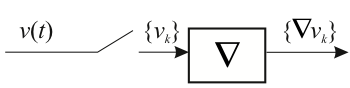
\includegraphics{pictures/cse1.png}}
  \end{center}
This can be represented in transform as
  \begin{center}
    \resizebox{180pt}{!}{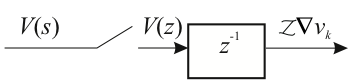
\includegraphics{pictures/cse2.png}}
  \end{center}
\endinput

\end{slide}
\fi
Consider a simple operation of sampling with a delay
  \begin{center}
    \resizebox{180pt}{!}{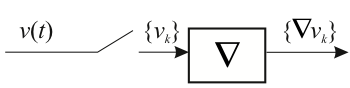
\includegraphics{pictures/cse1.png}}
  \end{center}
This can be represented in transform as
  \begin{center}
    \resizebox{180pt}{!}{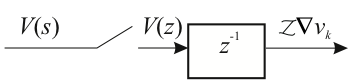
\includegraphics{pictures/cse2.png}}
  \end{center}
\endinput


\ifslidesonly
\begin{slide}\label{slide:l11s2}
  \heading{Sampling a Delayed Signal}
  The same result could be obtained by delaying the continuous
    signal and then sampling.
  \begin{center}
  \resizebox{180pt}{!}{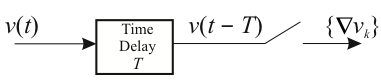
\includegraphics{pictures/cse3.png}}
  \end{center}
Which can be represented in transform as
  \begin{center}
   \resizebox{180pt}{!}{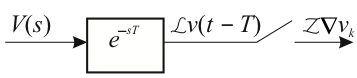
\includegraphics{pictures/cse4.png}}
  \end{center}
\endinput

\end{slide}
\fi
The same result could be obtained by delaying the continuous
    signal and then sampling.
  \begin{center}
  \resizebox{180pt}{!}{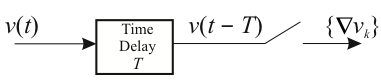
\includegraphics{pictures/cse3.png}}
  \end{center}
Which can be represented in transform as
  \begin{center}
   \resizebox{180pt}{!}{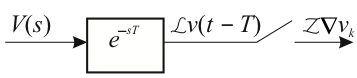
\includegraphics{pictures/cse4.png}}
  \end{center}
\endinput


\ifslidesonly
\begin{slide}\label{zisexpmst}
  \begin{equation}\label{eq:l12e1a}
	z=e^{sT}
\end{equation}
and
\begin{equation}\label{eq:l12e1b}
	s=\frac{1}{T}\ln z
\end{equation}
\endinput

\end{slide}
\fi
\begin{equation}\label{eq:l12e1a}
	z=e^{sT}
\end{equation}
and
\begin{equation}\label{eq:l12e1b}
	s=\frac{1}{T}\ln z
\end{equation}
\endinput


This is the fundamental relationship of equivalence. Before using it,
we must see how a continuous signal is reconstructed from a digital
signal. This is accomplished by means of a ``\emph{Digital-to-Analogue
Converter}''

\section*{Digital-to-Analogue Converter}

\ifslidesonly
\begin{slide}\label{dac}
\heading{Modelling a DAC with a Zero-Order Hold}
The simplest converter is a ``\emph{Zero-Order Hold}'' (see
Fig.~\ref{fig:l11f1}). This acts the opposite way to a sampler.
\begin{figure}[htbp]
  \begin{center}
    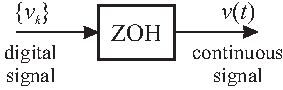
\includegraphics{pictures/zoh.pdf}
    \caption{Zero-Order Hold}
    \label{fig:l11f1}
  \end{center}
\end{figure}
\endinput

\end{slide}
\fi
The simplest converter is a ``\emph{Zero-Order Hold}'' (see
Fig.~\ref{fig:l11f1}). This acts the opposite way to a sampler.
\begin{figure}[htbp]
  \begin{center}
    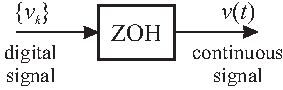
\includegraphics{pictures/zoh.pdf}
    \caption{Zero-Order Hold}
    \label{fig:l11f1}
  \end{center}
\end{figure}
\endinput


\ifslidesonly
\begin{slide}\label{dac}
\heading{Operaton of the Zero-order Hold}
During each sample period, the device holds the output $v(t)$ constant
at the current value of the digital signal $v_k$. That is
\begin{equation}
  \label{eq:l11e4}
  v(t) = v_k\ \mathrm{for}\ kT \le t < (k+1)T
\end{equation}
This generates a stepwise continuous signal $v(t)$ which at the
sampling instants is equal to the continuous signal from which the
digital signal ${v_k}$ was generated (\sref{slide:l11s3}).
\endinput

\end{slide}
\fi
During each sample period, the device holds the output $v(t)$ constant
at the current value of the digital signal $v_k$. That is
\begin{equation}
  \label{eq:l11e4}
  v(t) = v_k\ \mathrm{for}\ kT \le t < (k+1)T
\end{equation}
This generates a stepwise continuous signal $v(t)$ which at the
sampling instants is equal to the continuous signal from which the
digital signal ${v_k}$ was generated (\sref{slide:l11s3}).
\endinput


\begin{slide}\label{slide:l11s3}
  \heading{Step-wise continuous signal}
  This represents the output of the zero-order hold $v(t) = v_k$ for
  $kT \le t < (k+1)T$.\\
  \begin{center}
\resizebox{300pt}{!}{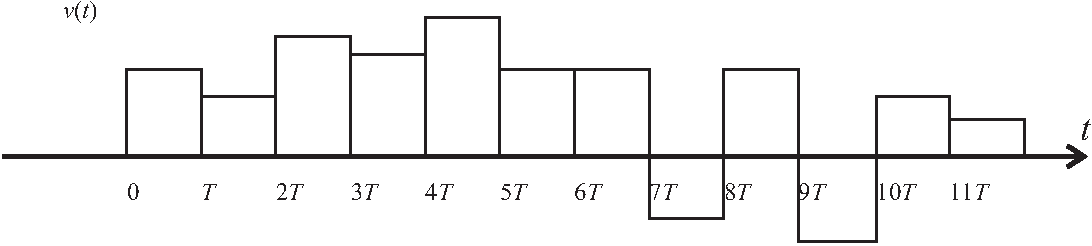
\includegraphics{pictures/steps.pdf}}
  \end{center}
\end{slide}

The signal may be considered as an infinite number of pulses of which
  the $k$-th is that shown in \sref{slide:l11s4}. To model such a
  signal we use the so-called ``\emph{gating}'' property of the
  time-delayed unit-step function $\epsilon(t)$ illustrated in \sref{slide:l11s5}.

\ifslidesonly
\begin{slide}
\heading{Modelling the ZOH Mathematically}
\end{slide}
\fi
\begin{slide}\label{slide:l11s4}
  \heading{The $k$-th ``Pulse''}
  \begin{center}
\resizebox{300pt}{!}{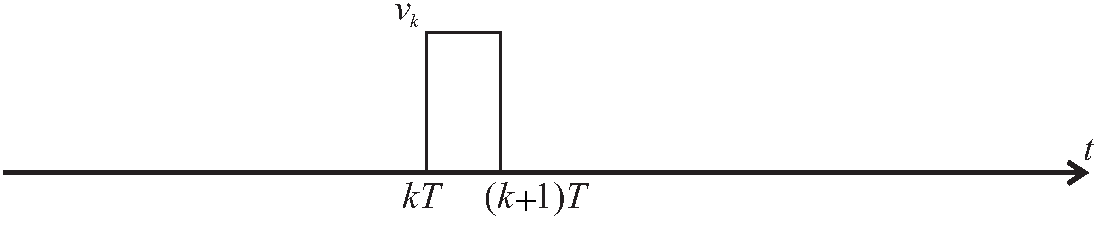
\includegraphics{pictures/pulse.pdf}}
  \end{center}
\end{slide}

\begin{slide}\label{slide:l11s5}
  \heading{The Gating Function (1)}
  \begin{center}
\resizebox{300pt}{!}{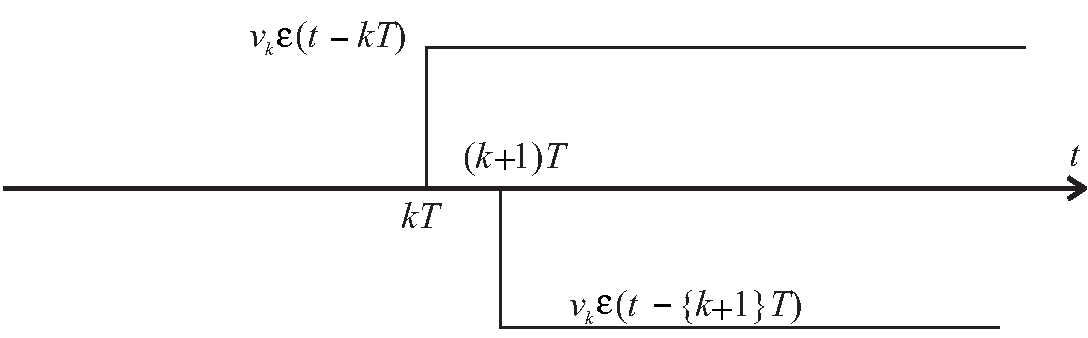
\includegraphics{pictures/gate.pdf}}
  \end{center}
\end{slide}

The opening ``gate'' is given by $v_k \epsilon (t-kT)$, a step of height
$v_k$, which is activated at $t=kT$ seconds. The gate is ``closed'' by
a negative going unit step, also of height $v_k$, which is activated
at $t=\{k+1\}T$ seconds.

\ifslidesonly
\begin{slide}
\heading{The Gating Function (2)}
The sum of these two signals is
\begin{eqnarray*}
  p(t) &=& v_k \epsilon(t - kT) - v_k \epsilon(t - \{k+1\}T)\\
       &=& v_k\left[\epsilon(t - kT) - \epsilon(t - \{k+1\}T)\right]
\end{eqnarray*}
So for the sequence:
\begin{equation}
  \label{eq:l11e5}
  v(t) = \sum_{k=0}^{\infty} v_k\left[\epsilon(t - kT) - \epsilon(t - \{k+1\}T)\right]
\end{equation}
\endinput

\end{slide}
\fi
The sum of these two signals is
\begin{eqnarray*}
  p(t) &=& v_k \epsilon(t - kT) - v_k \epsilon(t - \{k+1\}T)\\
       &=& v_k\left[\epsilon(t - kT) - \epsilon(t - \{k+1\}T)\right]
\end{eqnarray*}
So for the sequence:
\begin{equation}
  \label{eq:l11e5}
  v(t) = \sum_{k=0}^{\infty} v_k\left[\epsilon(t - kT) - \epsilon(t - \{k+1\}T)\right]
\end{equation}
\endinput


\ifslidesonly
\begin{slide}
\heading{The Gating Function (3)}
In transform form this is
\begin{eqnarray*}
  V(s) &=& \sum_{k=0}^{\infty} v_k\left(\frac{1}{s}e^{-kTs} -
  \frac{1}{s}e^{-\left\{k+1\right\}Ts}\right)\\
       &=& \frac{1}{s}\left(1-e^{-Ts}\right) \sum_{k=0}^{\infty} v_k
  e^{-kTs}\\
       &=& \frac{1}{s}\left(1-z^{-1}\right) \sum_{k=0}^{\infty} v_k
  z^{-k}\\
       &=& \frac{1}{s}\,\frac{z-1}{z}\,V(z)
\end{eqnarray*}
\endinput

\end{slide}
\fi
In transform form this is
\begin{eqnarray*}
  V(s) &=& \sum_{k=0}^{\infty} v_k\left(\frac{1}{s}e^{-kTs} -
  \frac{1}{s}e^{-\left\{k+1\right\}Ts}\right)\\
       &=& \frac{1}{s}\left(1-e^{-Ts}\right) \sum_{k=0}^{\infty} v_k
  e^{-kTs}\\
       &=& \frac{1}{s}\left(1-z^{-1}\right) \sum_{k=0}^{\infty} v_k
  z^{-k}\\
       &=& \frac{1}{s}\,\frac{z-1}{z}\,V(z)
\end{eqnarray*}
\endinput


\ifslidesonly
\begin{slide}
\heading{ZOH as mixed transfer function}
So the zero-order hold is represented by the mixed transfer function
\begin{equation}
  \label{eq:l11e10}
  G_{\mathrm{zoh}}=\frac{1}{s}\,\frac{z-1}{z}
\end{equation}
as shown in Fig.~\ref{fig:l11f2}.
\begin{figure}[htbp]
  \begin{center}
    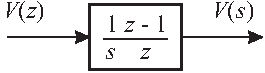
\includegraphics{pictures/zohtf.pdf}
    \caption{Transfer Function of the Zero-Order Hold}
    \label{fig:l11f2}
  \end{center}
\end{figure}
\endinput

\end{slide}
\fi
So the zero-order hold is represented by the mixed transfer function
\begin{equation}
  \label{eq:l11e10}
  G_{\mathrm{zoh}}=\frac{1}{s}\,\frac{z-1}{z}
\end{equation}
as shown in Fig.~\ref{fig:l11f2}.
\begin{figure}[htbp]
  \begin{center}
    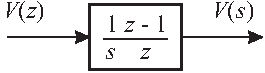
\includegraphics{pictures/zohtf.pdf}
    \caption{Transfer Function of the Zero-Order Hold}
    \label{fig:l11f2}
  \end{center}
\end{figure}
\endinput


\begin{slide}\label{slide:l11s10}
  \heading{Hold-Equivalent Digital System}
  \resizebox{300pt}{!}{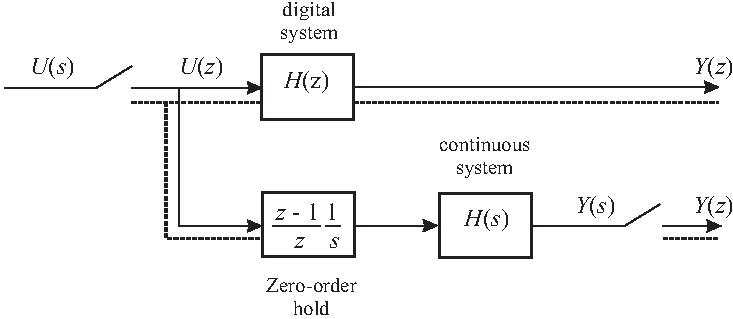
\includegraphics{pictures/holdequiv.pdf}}
\end{slide}

We can now design a `hold-equivalent' digital system.

\ifslidesonly
\begin{slide}
\heading{Hold-equivalent transform}
From the diagram in \sref{slide:l11s10}.
\begin{eqnarray*}
  Y(z) &=& H(z) U(z)\\
  Y(z) &=& \mathcal{Z} Y(s)\\
       &=& \mathcal{Z} \frac{1}{s} H(s) \frac{z-1}{z} U(z)
\end{eqnarray*}
so
\begin{eqnarray}\label{eq:l11e14}
  H(z) &=& \frac{z-1}{z} \mathcal{Z} \frac{H(s)}{s}
\end{eqnarray}
\endinput

\end{slide}
\fi
From the diagram in \sref{slide:l11s10}.
\begin{eqnarray*}
  Y(z) &=& H(z) U(z)\\
  Y(z) &=& \mathcal{Z} Y(s)\\
       &=& \mathcal{Z} \frac{1}{s} H(s) \frac{z-1}{z} U(z)
\end{eqnarray*}
so
\begin{eqnarray}\label{eq:l11e14}
  H(z) &=& \frac{z-1}{z} \mathcal{Z} \frac{H(s)}{s}
\end{eqnarray}
\endinput


\begin{slide}\label{slide:l11s11}
  \heading{Example 1}
  If \[H(s) = \frac{a}{s+a}\] then find the Zero-Order Hold Equivalent $H(z)$
\end{slide}

\subsubsection*{Solution}
\begin{eqnarray*}
  H(z) &=& \frac{z-1}{z}\mathcal{Z} \frac{a}{s(s+a)}\\
       &=& \frac{z-1}{z} \frac{z(1-e^{-aT})}{(z-1)(z-e^{-aT})}\\
       &=& \frac{1-e^{-aT}}{z-e^{-aT}}.
\end{eqnarray*}

\textbf{Malab note}: the zero-order-hold equivalent is the default
system used for continuous system equivalence in \emph{Matlab}. To
convert a continous system in any \emph{lti} format\footnote{%
The LTI functions are \emph{tf}, \emph{ss}, and \emph{zpk}. For more
information, type \emph{help lti} inside \emph{Matlab}.} use:
\begin{verbatim}
lti_d = c2d(lti, Ts); % You must provide a sampling time or use -1 if undefined
\end{verbatim}

\section*{Other Continuous System Equivalences}

\subsection*{Approximation based on numerical integration}

\ifslidesonly
\begin{slide}
\heading{Approximation based on numerical integration}
An alternative approach is to use the relationship \[ s  = \frac{1}{T}
\ln z. \] This cannot be substituted into a transfer function directly

Three approximations, obtained from numerical integration, may be
used.
as the result is not rational, but an approximation may be used.
\endinput

\end{slide}
\fi
An alternative approach is to use the relationship \[ s  = \frac{1}{T}
\ln z. \] This cannot be substituted into a transfer function directly

Three approximations, obtained from numerical integration, may be
used.
as the result is not rational, but an approximation may be used.
\endinput


\begin{slide}\label{slide:l11s20a}
  \heading{Approximation by Numerical Integration}
  \begin{itemize}
  \item We wish to find a transfer function $T(z)$ that is equivalent to $T(s)=s$.
  \item Let us instead seek a transfer function $D(z)$ that is equivalent to $D(s) = 1/s$.
  \end{itemize}
  \resizebox{300pt}{!}{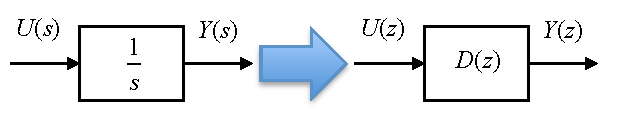
\includegraphics{pictures/s-to-z.pdf}}
\end{slide}

Thus, the transfer function we are seeking will in fact be an approximation of
the integral $y(t)=\int u(t) dt$. We can illustrate this as shown in SLIDE~\ref{slide:l11s20b}.
If we sample the curve $u(t)$ and consider the situation at the $n$-th sampling
instant, we will have $$y(nT) = \int_{0}^{nT} u(t) dt$$ We can rewrite this as
$$y(nT)= \int_{0}^{nT-T} u(t) dt + \int_{nT-T}^{nT} u(t) dt$$
where the second integral term is the shaded area shown in SLIDE~\ref{slide:l11s20c}.
Now if we assume that the first integral term was approximated by the digital
integrator in the previous sampling instant, then
$y(nT-T) = \int_{0}^{nT-T} u(t) dt$ is known, and consequently we have
$$y(nT) = y(nT-T) + \int_{nT-T}^{nT} u(t) dt$$
and we only need to determine the area of the shaded region to approximate $y(nT)$.

\begin{slide}\label{slide:l11s20b}
\heading{Model of Integration}
\begin{center}
	\resizebox{220pt}{!}{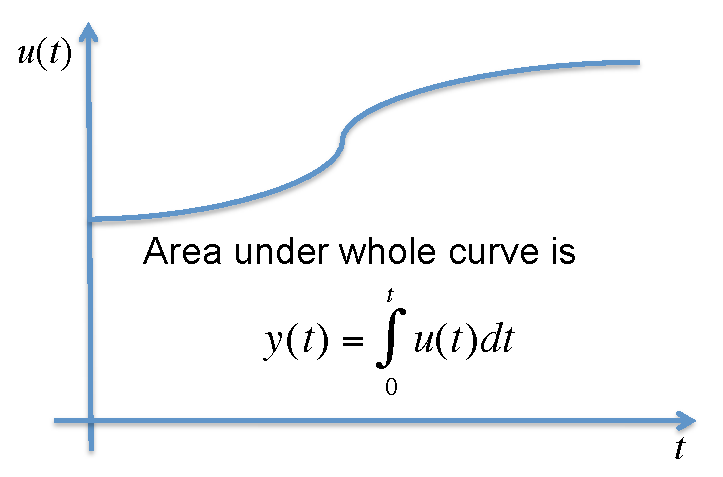
\includegraphics{pictures/integral1.pdf}}
\end{center}
\end{slide}

\begin{slide}\label{slide:l11s20c}
\heading{Sampled Model of Integration}
\begin{center}
	\resizebox{220pt}{!}{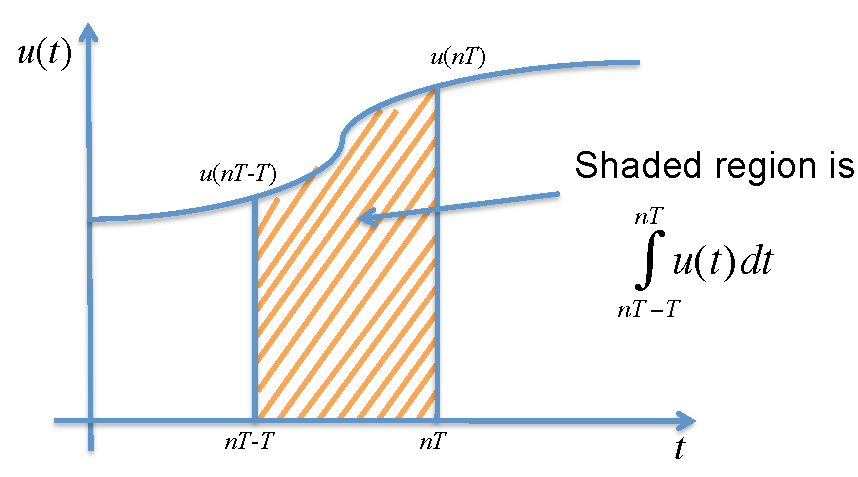
\includegraphics{pictures/integral2.pdf}}
\end{center}
\end{slide}

The most obvious approximations are illustrated in \sref{slide:l11s20d} to
\sref{slide:l11s20f}. It is clear that if we are to disallow any further
subdivision of the shaded area, the \emph{trapezoidal approximation}
will provide the most accurate result.

\begin{slide}\label{slide:l11s20d}
\heading{Forward Rectangular Approximation}
\begin{center}
	\resizebox{220pt}{!}{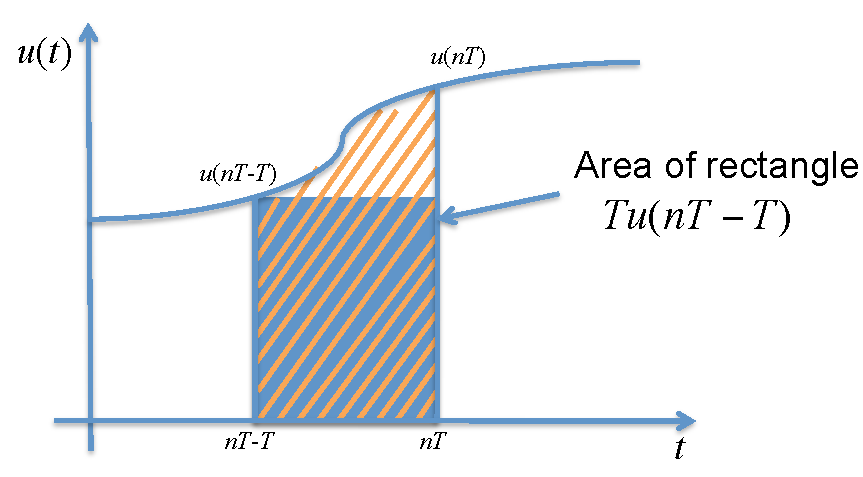
\includegraphics{pictures/forward-rect.pdf}}
\end{center}
\end{slide}

\begin{slide}\label{slide:l11s20e}
\heading{Backward Rectangular Approximation}
\begin{center}
	\resizebox{220pt}{!}{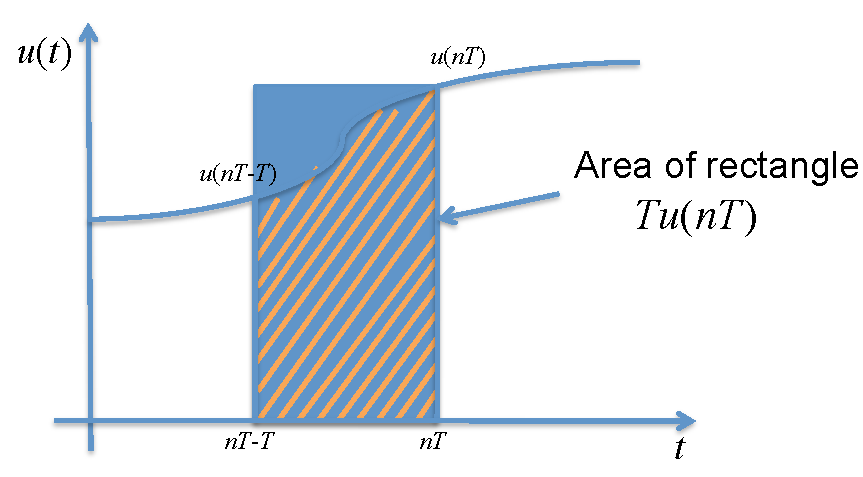
\includegraphics{pictures/backward-rect.pdf}}
\end{center}
\end{slide}

\begin{slide}\label{slide:l11s20f}
\heading{Trapezoidal Approximation}
\begin{center}
	\resizebox{220pt}{!}{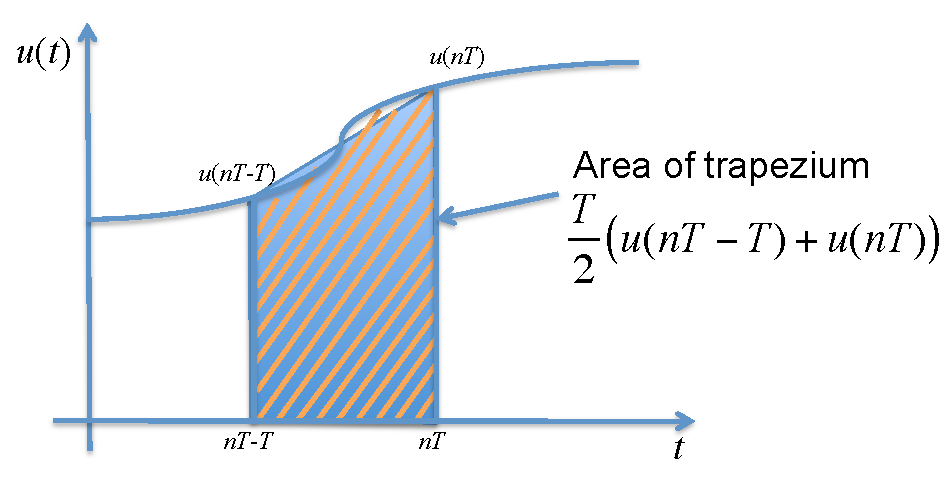
\includegraphics{pictures/trapezoidal.pdf}}
\end{center}
\end{slide}

\ifslidesonly
\begin{slide}
\heading{$z$-transform of trapezoidal approximation}
Completing the analysis, we can show that
$$y(nT)\approx y(nT-T) + \frac{T}{2}\{u(nT-T)+u(T)\}$$
which on taking z-transforms gives
$$Y(z)=z^{-1}Y(z)+\frac{T}{2}\{z^{-1}U(z)+U(z)\}$$
thus
\begin{equation}
\frac{Y(z)}{U(z)}=D(z)=\frac{T}{2}\left\{ {\frac{{1 + {z^{ - 1}}}}{{1 - {z^{ - 1}}}}} \right\}.
\end{equation}
\endinput

\end{slide}
\fi
Completing the analysis, we can show that
$$y(nT)\approx y(nT-T) + \frac{T}{2}\{u(nT-T)+u(T)\}$$
which on taking z-transforms gives
$$Y(z)=z^{-1}Y(z)+\frac{T}{2}\{z^{-1}U(z)+U(z)\}$$
thus
\begin{equation}
\frac{Y(z)}{U(z)}=D(z)=\frac{T}{2}\left\{ {\frac{{1 + {z^{ - 1}}}}{{1 - {z^{ - 1}}}}} \right\}.
\end{equation}
\endinput


\ifslidesonly
\begin{slide}
\heading{Approximation of $s$ by numerical integration}
The
response of a digital system with transfer function $H(z)$ to a
digital input signal $u$ is the digital output signal
$y$ given in transform form as
\begin{equation}\label{eq:l10e1}
  Y(z) =H(z) U(z)
\end{equation}
Taking the inverse transform gives the digital system response as
\begin{equation}\label{eq:l10e2}
  y_k = \mathcal{Z}^{-1}Y(z) = \mathcal{Z}^{-1} \left\{H(z)
  U(z)\right\}
\end{equation}
\endinput

\end{slide}
\fi
The
response of a digital system with transfer function $H(z)$ to a
digital input signal $u$ is the digital output signal
$y$ given in transform form as
\begin{equation}\label{eq:l10e1}
  Y(z) =H(z) U(z)
\end{equation}
Taking the inverse transform gives the digital system response as
\begin{equation}\label{eq:l10e2}
  y_k = \mathcal{Z}^{-1}Y(z) = \mathcal{Z}^{-1} \left\{H(z)
  U(z)\right\}
\end{equation}
\endinput


\begin{slide}\label{slide:l11s22}
  \heading{Trapezoidal Approximation}

  \begin{eqnarray*}
     s &=& \frac{2}{T}\, \frac{z-1}{z+1} \\
     z &=& \frac{1 + 1/2 sT}{1 - 1/2 sT}
  \end{eqnarray*}
  compare expansion $$z=(1+ (1/2) sT)(1- (1/2) sT)^{-1} = 1 + sT + (1/2)
 s^2T^2 + (1/4) s^3T^3
 + \cdots$$  with $$z = e^{sT} = 1 + sT + (1/2) s^2T^2 + (1/6) s^3T^3 + \cdots$$
\end{slide}

\begin{slide}\label{slide:l11s20}
  \heading{Forward Rectangular Approximation}

  \begin{eqnarray*}
     s &=& \frac{z-1}{T} \\
     z &=& 1 + sT
  \end{eqnarray*}
  compare with $$z = e^{sT} = 1 + sT + (1/2) s^2T^2 + (1/6) s^3T^3 + \cdots$$
\end{slide}

\begin{slide}\label{slide:l11s21}
  \heading{Backward Rectangular Approximation}

  \begin{eqnarray*}
     s &=& \frac{z-1}{Tz} \\
     z &=& \frac{1}{1 + sT}
  \end{eqnarray*}
  compare expansion $$z=(1-sT)^{-1} = 1 + sT + s^2T^2 + s^3T^3
 + \cdots$$  with $$z = e^{sT} = 1 + sT + (1/2) s^2T^2 + (1/6) s^3T^3 + \cdots$$
\end{slide}


The approximation shown in SLIDE\sref{slide:l11s22}) is
is known as ``\emph{Tustin's Bilinear Transformation}''.

\begin{slide}\label{slide:l11s23}
  \heading{Example 2}
  If \[H(s) = \frac{a}{s+a},\] determine the equivalent $H(z)$ using Tustin's
  bilinear transformation.
\end{slide}

\subsubsection{Solution}
Tustin's bilinear transformation gives a
 digital system with transfer function
 \begin{eqnarray*}
   H(z)&=& \frac{a}{\frac{2}{T}\,\frac{z-1}{z+1}+a} \\
       &=& \frac{\left(\frac{(aT)/2}{1+(aT)/2}\right)(z+1)}{z-\left(\frac{1-(aT)/2}{1+(aT)/2}\right)}.
 \end{eqnarray*}

\textbf{Malab note}: the bilinear transform equivalent is obtained by passing the argument \verb|'tustin'| to the \emph{c2d} method:
\begin{verbatim}
lti_d = c2d(lti, Ts, 'tustin');
\end{verbatim}

\subsection*{Matched pole-zero approximations}

Another way to obtain a digital approximation of a continuous transfer function
is to use the relationship $z = e^{sT}$ to map poles and zeros of the continuous
transfer function into poles and zeros in the z-transfer function.

Since continuous transfer functions often have more poles than zeros,
that is $n-m$ zeros at infinity, zeros at infinity are replaced in the z-transfer
function by zeros at $z = -1$ which is equivalent to half the sampling frequency
$\omega_s/2$ (i.e. the highest frequency possible in the z-domain).
Thus if $n-m =1$ we add $(1+z^{-1})$, if $n-m=2$, $(1+z^{-1})^2$, etc.

\begin{slide}\label{slides:l11s24}
	\heading{Matched-Pole Zero method}
	Idea is that all poles and zeros of continuous transfer function $D(s)$ can
  become poles and zeros of digital transfer function $D(z)$ if the mapping
  $z=e^{sT}$ is used.

	Method:
	\begin{enumerate}
		\item Map finite poles and zeros of $D(s)$ to poles and zeros of $D(z)$ according to $z=e^{sT}$.
		\item Add zeros at $z=-1$ for each infinite zero in $D(s)$.
		\item Match DC or low-frequency gain.
	\end{enumerate}
	See examples in the notes.
\end{slide}

\begin{slide}
\heading{Example 3}
Use the Matched-Pole-Zero (MPZ) approximation to give the z-transfer function equivalent to
$$D(s)=\frac{s+a}{s+b}.$$
\end{slide}
\subsubsection*{Solution}
Order of numerator and denominator are equal so there are no infinite zeros and
by matching poles and zeros
$$D(z)=k\frac{(1-e^{-aT}z^{-1})}{(1 - e^{-bT}z^{-1})}.$$
For $D(s)$ the DC gain is $D(s)|_{s=0} = a/b$.
The DC gain for $D(z)$ is $D(z)|_{z=1}$ (from final value theorem) that is
$$k\frac{(1-e^{-aT})}{(1-e^{-bT})} = \frac{a}{b}.$$
We choose $k$ so that the DC gains match, i.e.
$$k=\frac{a(1-e^{-bT})}{b(1-e^{-aT})}.$$

\begin{slide}
\heading{Example 4}

Use the Matched-Pole-Zero (MPZ) approximation to give the z-transfer function equivalent to
$$D(s)=\frac{s+a}{s(s+b)}.$$
\end{slide}

\subsubsection*{Solution}
Here, the order of the denominator is one greater than the numerator so there is
$n-m = 2 - 1 = 1$ infinite zero. Placing this zero at $z = -1$ makes the MPZ transfer
function
$$D(z)=k\frac{(1+z^{-1})(1-e^{-aT}z^{-1})}{(1-z^{-1})(1 - e^{-bT}z^{-1})}.$$
As $D(s)$ is type 1, we can't use the value of $D(0)$ to compute the DC gain.
Instead, let us compute the gain at $s = -1$:
\begin{eqnarray*}
  D( - 1) &=& {\left. {\frac{{s + a}}{{s(s + b)}}} \right|_{s =  - 1}} \\
   &=& \frac{{-1 + a}}{{( - 1)(-1 + b)}} = \frac{{a - 1}}{{(1 - b)}} \\
\end{eqnarray*}
The equivalent value $s=-1$ in the $z$-plane is $z=e^{-T}$.
\begin{eqnarray*}
  k{\left. {\frac{{(1 + {z^{ - 1}})(1 - {e^{ - aT}}{z^{ - 1}})}}{{(1 - {e^{ - bT}}{z^{ - 1}})}}} \right|_{z = {e^{ - T}}}} &=& k\frac{{(1 + {e^T})(1 - {e^{ - aT}}{e^T})}}{{(1 - {e^{ - bT}}{e^T})}} \hfill \\
   &=& k\frac{{\left( {1 + {e^T}} \right)\left( {1 - {e^{ - (1 - a)T}}} \right)}}{{\left( {1 - {e^{ - (1 - b)T}}} \right)}} \hfill \\
\end{eqnarray*}

Again, we choose $k$ so that the equivalent gains match, i.e.
$$k =  \left( {\frac{{1 - b}}{{a - 1}}} \right)\frac{{\left( {1 - {e^{ - (1 - b)T}}} \right)}}{{\left( {1 + {e^T}} \right)\left( {1 - {e^{ - (1 - a)T}}} \right)}}.$$

We would implement $D(z)$ as a \emph{difference equation} defined in terms of the
sampled inputs and outputs as shown in SLIDE~\ref{slides:l11s25} for Example 3.
\begin{slide}\label{slides:l11s25}
	\heading{Implementation of an MPZ Approximation}
	If $$\frac{Y(z)}{U(z)}=D(z)=k\frac{1-\alpha z^{-1}}{1-\beta z^{-1}}$$ then digital implementation will be
	$$y(n)=\beta y(n-1)+k(u(n)-\alpha u(n-1))$$
	$y(n)$ is the current calculated value, $y(n-1)$ is previous calculated value, $u(n)$ is current sample, and $u(n-1)$ is previous sample.

	Implementation only works if computation rate $<<$ significant dynamics of the sampled system and a small fraction of sampling time $T$.
\end{slide}

In the implementation, you should notice that it is actually physically impossible
to sample $u(t)$, compute $y(n)$ and output $y(n)$ all at the same instant of time.
Hence the equation is actually impossible to implement. However, if the
computation is sufficiently fast, the delay between sampling $u(t)$ and outputting
$y(t)$ will be small and can often be neglected.
A rule of thumb has computation delay $< t_r/20$ of the dominant pole.
It should certainly be a small fraction of the sampling period $T$.

\begin{slide}\label{slides:l11s26}
	\heading{Modified MPZ}
	\begin{itemize}
	\item
	Used if constraint on computation time cannot be met\footnote{Which these days is unlikely}.

	\item Allow a zero at infinity in $D(z)$ so that order of numerator is one
  less than denominator.

	\item This ensures that only past values of $u$ and $y$ appear in the implementation
  equation and a whole sample period is available for computation

\end{itemize}
\end{slide}

\begin{slide}\heading{Example 5}

Re-implement Example 3 using the Modified MPZ method.
\end{slide}
\subsubsection*{Solution}
If we allow an infinite zero
$$D(s)=\frac{s+a}{s(s+b)}$$ becomes
$$D(z)=k\frac{(1-e^{-aT}z^{-1})}{(1-z^{-1})(1-e^{-bT}z^{-1})}$$ and
$$k = \left( {\frac{{1 - b}}{{a - 1}}} \right)\frac{{\left( {1 - {e^{ - (1 - b)T}}} \right)}}{{\left( {1 - {e^{ - (1 - a)T}}} \right)}}.$$

The implementation is now

$$y(n) = (1 - e^{-bT})y(n-1)-e^{-bT}y(n-2)+k(u(n-1)-e^{-aT}u(n-2))$$

and now the computation for $y(n)$ is performed only on past values of $u(n)$ and
$y(n)$ and a whole sample period is available for computation.

\textbf{Matlab note}: the matched-pole zero equivalent of an LTI system is obtained by passing \verb|'matched'| as the third argument to \emph{c2d}:
\begin{verbatim}
lti_d = c2d(lti, Ts, 'matched')
\end{verbatim}
There isn't a built-in method that returns the \emph{modified}-matched-pole zero equivalent.


%----------------------------------------------------------------
% The end of notes
% ----------------------------------------------------------------
\endinput

% Local Variables:
% TeX-master: "lecture03"
% End:
